\documentclass{article}

\usepackage{graphicx}

\begin{document}

\title{Homework2}
\author{Qi Mao\\
  \texttt{maoxx241@umn.edu}}
\maketitle


\section{Question1:}
What are the disadvantages of using a heuristic function for A* which is not consistent? Be precise and provide an example to support the points you are making. \hbadness=99999
\break

an inconsistent heuristic function is h(x)$>$c(x,y)+h(y). the disadvantages of using inconsistent heuristic function is that the algorithm
will expand more node. And it will cause the algorithm hard to choose the optimal
solution.\newline
For example, there is a graph. If the heuristic function is inconsistent, it will hard to find the optimal solution to Goal.
\begin{center}
    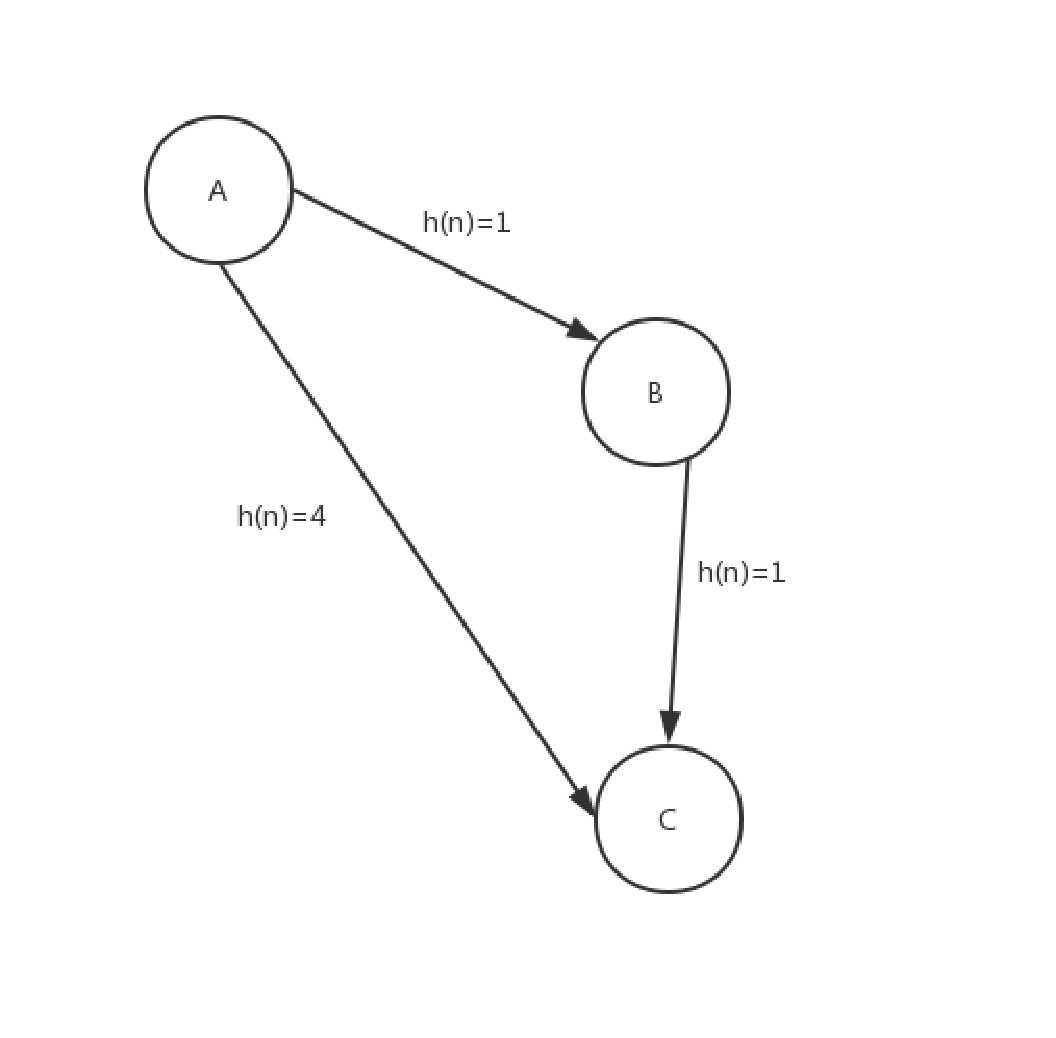
\includegraphics[scale=0.5]{2}
\end{center}

\section{Question2:}
The functions g and h each play a different role in A*. What are those roles? What happens when you emphasize or de-emphasize one of them by using different weights in f(n)? Consider the case in which f(n) = (1 - w)g(n) + wh(n), with 0 $\leq$ w $\leq$ 1. Be specific and analyze what happens for different values of w. \hbadness=99999

g(n): the cost from initial state to n.\newline \hbadness=99999
h(n): the estimate cost form h to the gaol.\newline
When I emphasize one of them, the algorithm will choose the different strategy to find the
the path to goal.\newline
when w = 0, then f(n)=g(n), then the algorithm becomes to Uniform Cost search, and it will just find the optimal path which has the samllest cost from
initial state to goal \newline
when 0$<$w$<$0.5, the prioirty of g(n) is heigher than h(n), it has more probability to find the optimal solution. \newline
when w = 0.5, then the function will not be changed.\newline
when 0.5$<$n$<$1, the prioirty of h(n) is heigher than g(n), it has less probability to find the optimal solution. \newline
when w = 1, then f(n)=h(n), then the algorithm will find the path which has the samllest heuristic estimate cost form initial state to goal. And it will not guarantee to find the optimal solution.\newline

\section{Question3:}
Discuss the possible advantages of the following state-space search strategy: obtain by some method a path to a goal node and its associated cost f(Goal)=C. This cost is not necessarily minimal but it gives an upper bound on the minimal cost. Now use A* with an admissible $h$ function and discard immediately any OPEN nodes reached whose f values are greater than C.

\begin{itemize}
	\item \texttt{1.}Explain if the modified A* algorithm with this strategy is guaranteed to find an optimal solution if one exists or not. Be short but precise.
    
    It depends on the data is tree or graph. If the data is tree, the algorithm will guarantee an optimal solution.
    Beuase when the heuristic function is admissible, the search algorithm will guarantee an optimal solution.
    When the data type is graph, if the heuristic is inconsistent, the search algorithm will not guarantee an optimal solution.
    
\end{itemize}


\begin{itemize}
    \item \texttt{2.}Explain if the fact that the algorithm discards some of the OPEN nodes (i.e. nodes in the frontier) means that fewer nodes are expanded. Be short but precise.
    
    No. when the algorithm discards some of the OPEN nodes, it means the f(n) of node is larger
    then C*. A* expands all nodes with f(n) $\leq$ C*.
    

\end{itemize}

\begin{itemize}
    \item \texttt{3.}Does this strategy reduce the total storage requirements? Explain your reasoning.
    
    Yes. Because it will discard the code is larger than C*. this operation will save the memory.

\end{itemize}





\section{Question4:}
Answer the following questions on Uniform Cost search briefly but precisely:

\begin{itemize}
	\item \texttt{1.}Is it possible for Uniform Cost to expand more nodes than Depth-First search? Feel free to use an example to support your answer.\newline
    Yes. For example,if I want from A to C. when I use Depth-First search, it will only expand A to C. If I use Uniform Cost, it will expand A to C and A to B.
    \begin{center}
        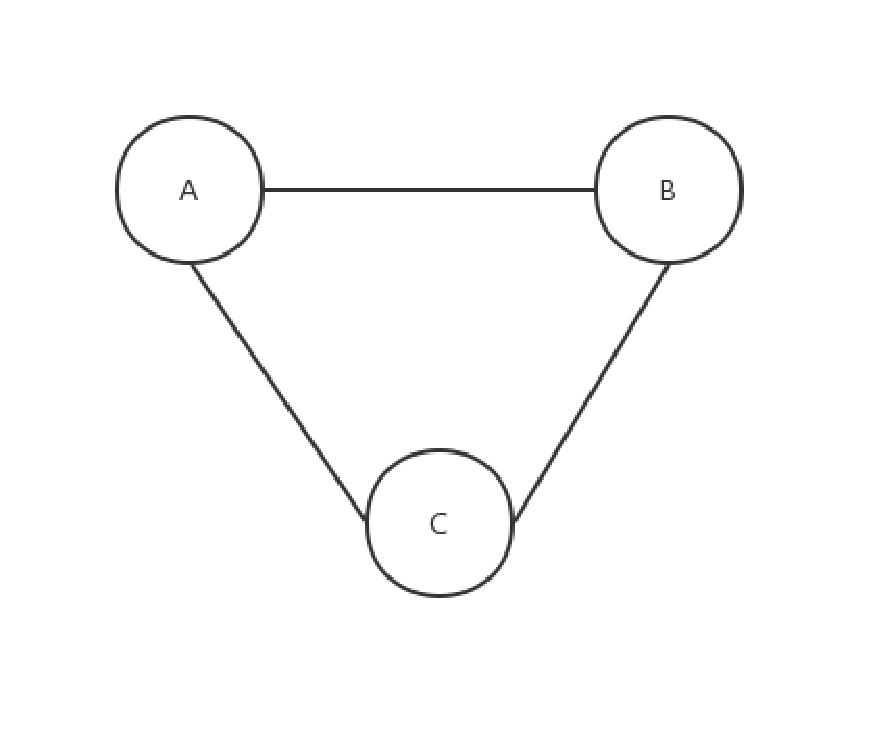
\includegraphics[scale=0.5]{1}
    \end{center}
\end{itemize}

\begin{itemize}
    \item \texttt{2.}Does Uniform Cost search expand more nodes than A*? Why (or why not)?\newline
    Yes. From the book page 93:\newline
    "The algorithm is identical to UNIFORM-COST-SEARCH except
    that A* uses g + h instead of g."\newline
    At most times, the heuristic function is admissible and consistent, so the Uniform Cost search will expanded less nodes than 
    A*.
\end{itemize}




\section{Question5:}
Answer the following questions explaining your reasoning briefly but precisely.

\begin{itemize}
	\item \texttt{1.}Why any node in OPEN with f(n) $<$ $f^*(n)$ (the cost of the optimal solution path) will eventually be selected for expansion by A*?\newline
    
    From the book page 97, we have: \newline If C* is the cost of the optimal solution path, then we can say the following:\newline
• A* expands all nodes with f(n) $<$ C*.\newline
• A* might then expand some of the nodes right on the “goal contour” (where f(n) = C*)\newline
before selecting a goal node.
Completeness requires that there be only finitely many nodes with cost less than or equal to
C*, a condition that is true if all step costs exceed some finite  and if b is finite.\newline



\end{itemize}

\begin{itemize}
    \item \texttt{2.}Is it true that all admissible heuristics are equal in the sense that A* will search the states in the same order no matter what the heuristic is?\newline
    
    No. If the heuristic function is calculate the distance from the node to goal for a map question. It will cause
    the algorithm go straight form initial state to goal.
\end{itemize}

\begin{itemize}
    \item \texttt{3.}Is Breadth-First search complete if the state space has infinite depth but a finite branching factor?
    
    Yes. Because the Breadth-First search will complete the level then move to next level. If there is a goal in some level,
    the Breadth-First search will reach the level and it will find the goal.
\end{itemize}

\begin{itemize}
    \item \texttt{4.}Does the fact that A* is ``optimally efficient'' mean that A* will never expand more nodes than any other algorithm?
    
    No. The garantee is therefore dependent of the heursitic garantee. If the heuristics function is not consistent and admissible, A* will expand more nodes.
    Form book page 98, we have:\newline
    One final observation is that among optimal algorithms of this type—algorithms that
extend search paths from the root and use the same heuristic information—A* is optimally
efficient for any given consistent heuristic. That is, no other optimal algorithm is guaran- 
teed to expand fewer nodes than A* (except possibly through tie-breaking among nodes with
f(n) = C*). This is because any algorithm that does not expand all nodes with f(n) $<$ C*
runs the risk of missing the optimal solution.\newline
    This is not prove that A* is always expand the least node than other algorithms.
\end{itemize}

\end{document}